\chapter*{Management Summary}
\thispagestyle{scrheadings}
% Titel auch in Kopfzeile anzeigen
\markboth{Management Summary}{Management Summary}

\todo[inline]{Gamification Konzept für OpenStreetMap aus Dokumentation entfernen}

\section*{Ausgangslage}
Das \brand{OpenStreetMap}-Projekt beinhaltet eine sehr grosse Menge an Daten, welche frei zugänglich ist.
Für die Pflege dieser Daten ist es daher naheliegend, auf unterstützende Software zurückzugreifen.
Zu diesem Zweck gibt es eine Reihe von Applikationen, welche sich grob in zwei Kategorien einteilen lassen:
Editoren und Tools zur Qualitätssicherung.

Mit den Editoren lässt sich direkt oder indirekt die \brand{OpenStreetMap}-Karte verändern und ergänzen.
Die Qualitätssicherungstools haben sich zum Ziel gesetzt, fehlende oder falsche Daten aufzuspüren.
Diese werden dann entweder automatisch korrigiert oder übersichtlich dargestellt, um eine manuelle Korrektur zu ermöglichen.

Einige Tools wie \brand{KeepRight}\footnote{\url{http://keepright.ipax.at/}} oder \brand{Osmose}\footnote{\url{http://osmose.openstreetmap.fr/map/}} (Abbildung \ref{image-osmose-screenshot}) berechnen aus den Karten-Rohdaten die vorhandenen Fehler.
Dazu werden einige Heuristiken verwendet oder einfache Plausibilitätsprüfungen durchgeführt.
Typische Fehler aus diesen Quellen sind \glspl{POI} ohne Namen oder Strassen ohne definierte Geschwindigkeitslimiten.

\begin{figure}[H]
	\centering
	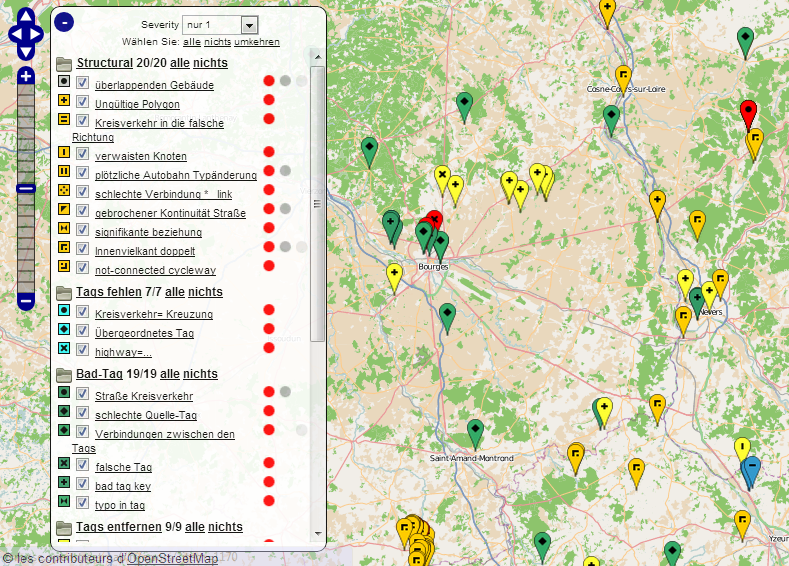
\includegraphics[scale=0.4]{images/managementsummary/osmose-screenshot}
	\caption{Anzeige von generierten Fehlern in Osmose}
	\label{image-osmose-screenshot}
\end{figure}

Andere Lösungen setzen darauf, dass Fehler manuell von einer Person erfasst werden. Dadurch ist es möglich, den Fehler detaillierter zu beschreiben. 
So gibt es Navigationsgeräte-Hersteller, welche die Daten aus \brand{OpenStreetMap} zur Routenberechnung verwenden, und dabei ihren Benutzern ermöglichen, falsche Routen zu melden.

Falls ein \gls{Mapper} einen Fehler melden will, so kann er diesen direkt in den Metadaten der Karte hinterlegen. Alle Objekte auf der Karte (Punkte, Wege und Relationen) können durch beliebige, sogenannte  \glspl{Tag} ergänzt werden.
Um auf einem Objekt Fehler zu markieren, hat sich die Community darauf geeinigt, dafür \inlinecode{FIXME}-\glspl{Tag} zu verwenden.

Quellen für derartige Fehler sind beispielsweise \brand{OpenStreetBugs}\footnote{\url{http://openstreetbugs.schokokeks.org/}} oder die \inlinecode{FIXME}-\glspl{Tag} aus \brand{KeepRight}.

\section*{Ergebnisse}
Das Ziel, eine plattformübergreifende \gls{WebApp} zu erstellen mit geeignetem Backend für die Verwaltung der Daten, wurde klar erreicht.
Die App bietet alle Grundfunktionalitäten, welche nötig sind, um Fehler anzuzeigen, zu lösen und gegebene Vorschläge zu validieren.
Daneben sind einige Elemente der \gls{Gamification} implementiert. So ist es beispielsweise möglich, durch das Lösen von Fehlern Punkte (sogenannte \emph{Koins}) zu sammeln und sich über eine Highscore mit anderen Spielern zu messen.
Zudem gibt es für speziellen Einsatz Auszeichnungen zu gewinnen.

\begin{figure}[H]
	\centering
	
\includegraphics[scale=0.6]{images/gamification/gamification-badges}
	\caption{Auszeichnungen in Kort}
	\label{image-kort-badges}
\end{figure}

Der Bereich der \gls{Gamification} ist aber sehr offen und lässt Raum für viele weitere Konzepte. Schlussendlich ist jedoch klar, dass \textsc{Kort} noch ein Stück davon entfernt ist, ein "`echtes"' Game zu sein.

Das Themengebiet der \gls{Gamification} bietet viele Ansätze, um repetitive Aufgaben spannend zu gestalten.
Dadurch erhalten diese einen ganz neuen Reiz und sprechen den Spieltrieb des Menschen an.
Konkret auf \brand{OpenStreetMap} angewendet, finden sich auch dort beliebtere und weniger beliebte Aufgaben.
Da es sich dabei zusätzlich um eine Community von freiwilligen Personen handelt, verschärft sich dieses Problem.
Das Problem der mangelnden Ressourcen kann dabei am effektivsten bekämpft werden, indem zusätzliche Personen für das Thema begeistert werden.
Für diese Zielgruppe braucht es neue Werkzeuge, die einfach zu bedienen sind und Spass machen.\todo{Abschnitt überarbeiten. Jetzt ok?}

\subsection*{Frontend}
Das Frontend basiert auf dem HTML5/JavaScript Framework \brand{Sencha Touch 2} und orientiert sich vom Look and Feel an einer iPhone-App.
Die App bietet für die verschiedenen Funktionen unterschiedliche Tabs an, in welchen der Benutzer Fehler beheben oder prüfen und die Rangliste oder sein Profil anschauen kann.

\begin{figure}[H]
\subfigure{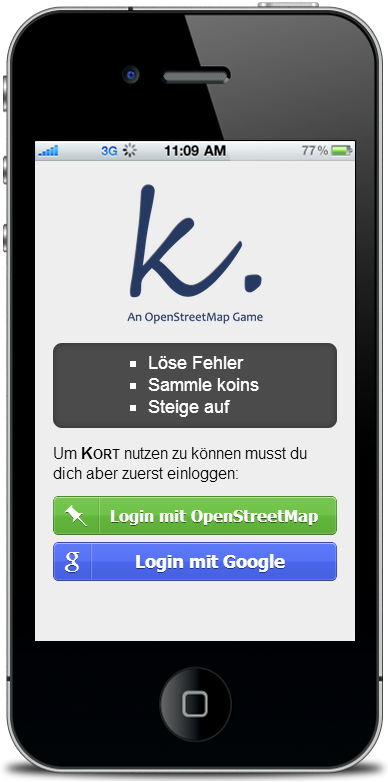
\includegraphics[width=0.3\textwidth]{images/screenshots/kort-screenshot-login}}
\hfill
\subfigure{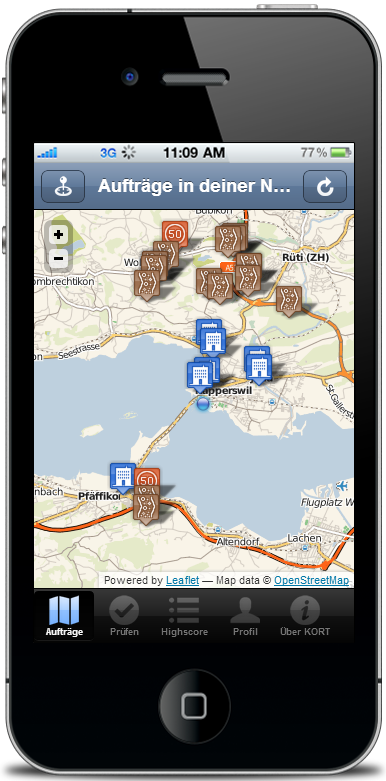
\includegraphics[width=0.3\textwidth]{images/screenshots/kort-screenshot-bugmap}}
\hfill
\subfigure{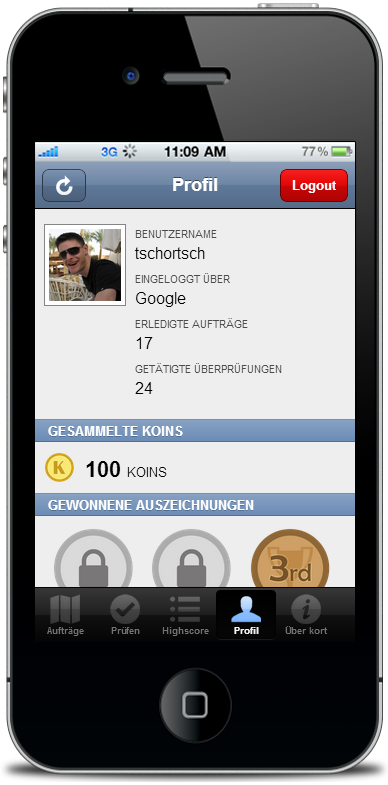
\includegraphics[width=0.3\textwidth]{images/screenshots/kort-screenshot-profile}}
\caption{\kort{} App}
\label{image-kort-screenshots}
\end{figure}

Für die Authentifizierung kommt \gls{OAuth} zum Einsatz.
Der Standard sorgt dafür, dass sich der Benutzer mit einem bereits bestehenden Benutzerkonto bei \textsc{Kort} anmelden kann.
Derzeit werden dafür die \gls{OAuth}-Provider \brand{OpenStreetMap} und \brand{Google} verwendet.

\subsection*{Backend}
Das Backend ist in PHP geschrieben und basiert auf der Kommunikation über \gls{REST}-Schnittstellen.
Die eigenen Schnittstellen sind alle mit dem \brand{Slim-Framework}\footnote{\url{http://www.slimframework.com/}} erstellt.
Da die Datenbank und der Webserver auf zwei verschiedenen Servern laufen, bietet auch die Datenbank eine \gls{REST}-Schnittstelle an, über welche sich beliebige SQL-Abfragen absetzen lassen.
Diese flexible Aufteilung ermöglicht es sehr einfach, die Systeme zu migrieren oder weitere hinzuzufügen.

\section*{Ausblick}
Die App hat grosses Potential, Personen, welche sich bislang nicht mit der Thematik \brand{OpenStreetMap} befasst haben, für das Projekt zu begeistern.

Ganz allgemein ist es wichtig, die Robustheit und Geschwindikeit der App zu verbessern. 
Gerade weil es sich um eine \gls{WebApp} handelt, ist dies besonders kritisch. 
Im Idealfall sollte sich die App nicht von einer nativen App unterscheiden.
Es ist zu prüfen, ob es sich lohnt, die App native zu bilden\footnote{z.B. mit Apache Cordova oder Sencha Packager}.
Dies hätte den Vorteil, dass die App über die bekannten \glspl{App-Store} zum User gebracht werden kann.

Beim Login wäre es wünschenswert, noch weitere \gls{OAuth}-Dienste anzubieten, um so weitere Personen anzusprechen und die Akzeptanz zu steigern.
Schliesslich verfügt nicht jeder über ein \brand{OpenStreetMap}- oder ein Google-Konto.
Mögliche Dienste sind beispielweise Facebook oder Twitter, welche beide \gls{OAuth} anbieten.

Um die Validierung von Lösungsvorschlägen zu verbessern, wäre es wünschenswert wenn ein Benutzer direkt einen Fotobeweis anbringen könnte.
Dies hilft die Datenqualität hoch zu halten und macht eine Änderung leichter überprüfbar.
Der Benutzer könnte dafür beispielsweise mit zusätzlichen Punkten belohnt werden.
Technisch wäre es sicher spannend sich mit dem \gls{Camera API} auseinander zu setzen.

Als zusätzliche Motivation könnten zeitlich begrenzte Aktionen durchgeführt werden.
Dies soll Benutzer dazu animieren, die App immer wieder zu verwenden. 
Mögliche Aktionen wären beispielsweise die Konzentration auf einen Fehlertyp (\emph{"`Gib allen Restaurants in deiner Umgebung einen Namen und erhalte diese Woche die spezielle Restaurant-Auszeichnung"'}) oder auf eine Region (\emph{"`Korrigiere jeden Tag im Dezember Fehler in Zürich und erhalte die Zürich-Silvester-Auszeichnung"'}).
Die Spieler könnten beispielsweise mittels Push-Notifikationen über solche Aktionen oder sonstige Neuerungen informiert werden.

Um die App längerfristig am Laufen zu halten, ist es unumgänglich, weitere Fehlertypen und -quellen einzubinden. 
\brand{KeepRight} bietet zwar eine grosse Menge an Fehlerdaten, jedoch ist nur ein geringer Teil davon für unsere App nutzbar.

Die Bekanntheit der App muss durch geeignete Massnahmen gesteigert werden. Dazu gehört die Integration von Social Media-Diensten wie Facebook und Twitter.
Diese kann einerseits genutzt werden, um Werbung zu machen, anderseits können Benutzer auf bereits gewonnene Auszeichnungen aufmerksam gemacht werden und so dazu animieren, diese Auszeichnungen ebenfalls zu gewinnen.
Ähnlich wie man es von anderen Apps wie beispielsweise \brand{Foursquare}\footnote{\url{https://foursquare.com/}} oder \brand{SBB.Connect}\footnote{\url{http://www.sbb.ch/fahrplan/mobile-fahrplaene/mobile-apps/sbb-connect.html}} kennt.

Die wichtigste, noch offene Erweiterung stellt aber das noch fehlende Zurückschreiben der eingetragenen Lösungen zu \brand{OpenStreetMap} dar.
Diese Funktionalität wirkt sich stark auf die Akzeptanz der App seitens der \brand{OpenStreetMap}-Community aus.